\documentclass[12pt]{article}

\usepackage[utf8]{inputenc}
\usepackage[brazil]{babel}
\usepackage[a4paper,left=3cm, right=2cm,top=2.5cm, bottom=2.5cm]{geometry}
\usepackage{amsmath}
\usepackage{graphicx}
\usepackage{float}
\usepackage{multirow}
\usepackage{authblk}
\usepackage{fancyhdr}
\usepackage{xcolor}
\usepackage{cite}


\title{\textbf{ENG1456 - Redes Neurais - Trabalho 2 Previsão de Séries Temorais}}
\author{\textbf{Aluno: Matheus Carneiro Nogueira - 1810764}}
\affil{}
\author{\textbf{Professora: Marley Velasco}}
\affil{}
\pagestyle{fancy}
\fancyhf{}
\lhead{{\small \textcolor{gray}{PUC-Rio ENG1456}}}
\renewcommand{\headrulewidth}{0pt}
\date{}
\renewcommand{\footrulewidth}{0pt}
\fancyfoot[C]{\thepage}

\begin{document}
	\maketitle
	\tableofcontents
	
	
	\begin{abstract}
		Este documento consiste no relatório do trabalho 2 do módulo de Redes Neurais da disciplina ENG1456 da PUC-Rio. Nele será explicada a implementação de modelos de Redes Neurais MLP para a previsão de uma série temporal do dataset MicroClima2 , disponibilizado pela professora da disciplina. A seções do relatório são definidas de acordo com as perguntas principais que constam no arquivo Guia de Atividades II. Foram consultados os materiais de aula, o livro \cite{livro} e outros materiais devidamente referenciados.
	\end{abstract}
		
	\section{Compreensão do Problema}
	\subsection{Visualize, em forma de gráfico, a dinâmica temporal da série escolhida. A série é adequada para a modelagem usando Redes Neurais? Caso não seja, que técnicas podem ser aplicadas para ajustar o comportamento da série?}\label{subsec:1.1}
	
	A série utilizada neste trabalho, denominada \textit{microclima2} consiste em 144 temperaturas média mensais, ou seja, temos informação sobre as temperaturas dos últimos 12 anos.
	
	Com o intuito de analisar a dinâmica temporal da série, foi gerado o gráfico da série em si e da decomposição dela, com o intuito de verificar \textit{trending} e \textit{sazonalidade}. As figuras abaixo ilustram esses resultados.
	
	\begin{figure}[H]
		\centering
		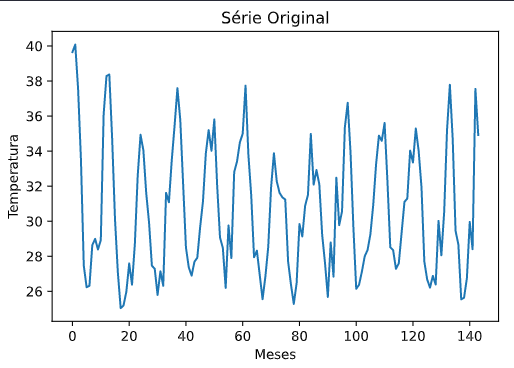
\includegraphics[width=0.7\linewidth]{Imagens/serieoriginal/plotserie}
		\caption{Série Original}
		\label{fig:plotserie}
	\end{figure}
	\begin{figure}[H]
		\centering
		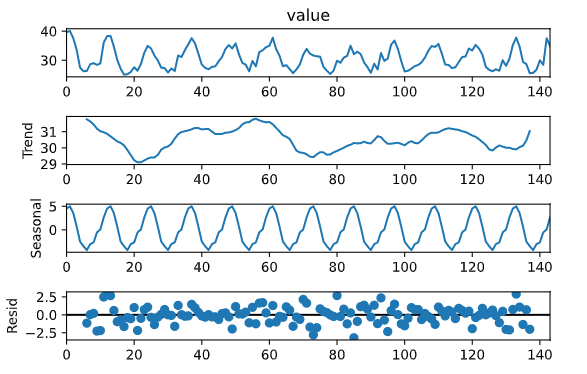
\includegraphics[width=0.7\linewidth]{Imagens/serieoriginal/decomposeSerie}
		\caption{Decomposição da Série Original}
		\label{fig:decomposeserie}
	\end{figure}

	Ao analisar a figura \ref{fig:plotserie} notamos que a série possui um perfil estacionário ao longo dos 12 anos. Isso quer dizer que a temperatura média de cada mês do ano \textit{a} é similar à temperatura média de cada mês no ano \textit{a+1}. Além disso, a figura \ref{fig:decomposeserie} revela, em seu campo \textit{Trend}, a tendência da série ao longo do tempo. Embora existam oscilações nesse gráfico, não se percebe nenhuma tendência geral da série. Com o intuito de ir além da análise visual, foi executado o \textit{Augmented Dickey-Fuller test} para verificar a probabilidade de existência de uma raiz unitária, que indicaria perfil não estacionário. O resultado é expresso na figura abaixo.
	\begin{figure}[H]
		\centering
		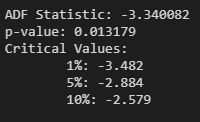
\includegraphics[width=0.5\linewidth]{Imagens/serieoriginal/asfteste}
		\caption{ADF Test}
		\label{fig:asfteste}
	\end{figure}
	
	Nota-se que o \textit{p-value} é muito pequeno e que o valor de \textit{ADF Statistic} é menor que o valor crítico para 1\%. Isso indica que esta série possui probabilidade baixíssima a alto grau de confiança em relação à inexistência de uma raiz unitária. Sendo assim, podemos tratá-la como uma série estacionária. Essa análise é importante pois, caso a série fosse não-estacionária, a rede neural precisaria, além de aprender o andamento temporal da série, aprender também a sua tendência, o que aumentaria a complexidade do modelo. Para corrigir esse problema, poderíamos tornar a série estacionária por meio de uma diferenciação, por exemplo, lembrando, apenas, de voltar aos valores originais ao final.
	
	Como a série em questão possui valores de temperaturas médias mensais ao longo dos anos, é de se esperar que exista uma sazonalidade razoavelmente perceptível. Ambas as figuras \ref{fig:plotserie} e \ref{fig:decomposeserie} mostram que essa sazonalidade existe de fato. Com essas imagens em mãos e supondo que o mês 1.0 é Janeiro, podemos inferir que as temperaturas referem-se a um local do hemisfério sul, onde é verão em janeiro, uma vez que as maiores temperaturas encontram-se próximas desse mês. Essa informação (o mês da temperatura) será útil para o treinamento da série, portanto deve constar nos dados de entrada. Como a sazonalidade não oferece problemas para a modelagem com um \textit{MLP}, não precisamos fazer nenhum tipo de correção.
	
	
	\subsection{No problema escolhido, usaremos uma variável exógena que representa	o mês de previsão (i.e. no instante t+1). De que forma esta variável pode auxiliar na previsão da série temporal?}
	
	Como comentado na seção \ref{subsec:1.1}, a série de temperaturas apresenta sazonalidade anual, isto é, o perfil de evolução da séria se repete de ano em ano, o que é de se esperar dada a natureza da série. Desse modo, fornecer o mês do valor de entrada pode auxiliar bastante na qualidade da previsão da série, uma vez que meses como Dezembro a Fevereiro (12 a 3) geralmente apresentam temperaturas médias mais altas, enquanto meses como Maio a Setembro (5 a 9) apresentam temperaturas mais baixas. Ao fornecer essa informação para Rede Neural, ela possuirá mais informações para aprender o perfil de sazonalidade da série, aumentando sua qualidade de previsão. 
	
	\section{Previsão One-Step}
	
	\subsection{Execute o script para a previsão one-step. Analise o resultado (conjunto	de treinamento e teste), usando as métricas RMSE e MAE.}\label{subsec:2.1}
	
	Para realizar a previsão de um passo à frente, foram testadas diversas configurações de redes neurais, variando a quantidade de neurônios na camada escondida. Os erros \textit{RMSE} e \textit{MAE} de cada uma dessas configurações estão apresentados na tabela a seguir. Vale comentar que, no arquivo \textit{jupyter notebook} enviado junto deste relatório está presente apenas o modelo final escolhido. Além disso, o script definia a métrica \textit{MSE}, então,para obter a métrica desejada, \textit{RMSE} foi calculada a raiz quadrada da \textit{MSE} fornecida.
	
	\begin{table}[H]\label{tab:comparacaoNeuronios}
		\centering
		\begin{tabular}{|l|l|l|l|l|l|l|}
			\hline
			\# neurônios & 5     & 10    & 15    & 20    & 25    & 30    \\ \hline
			RMSE         & 3.007 & 2.871 & 3.022 & 2.584 & 2.598 & 2.936 \\ \hline
			MAE          & 2.090 & 2.105 & 2.434 & 1.938 & 1.968 & 2.343 \\ \hline
		\end{tabular}
	\caption{Comparação dos Erros para diferentes números de neurônios}
	\end{table}

	\begin{figure}[H]
		\centering
		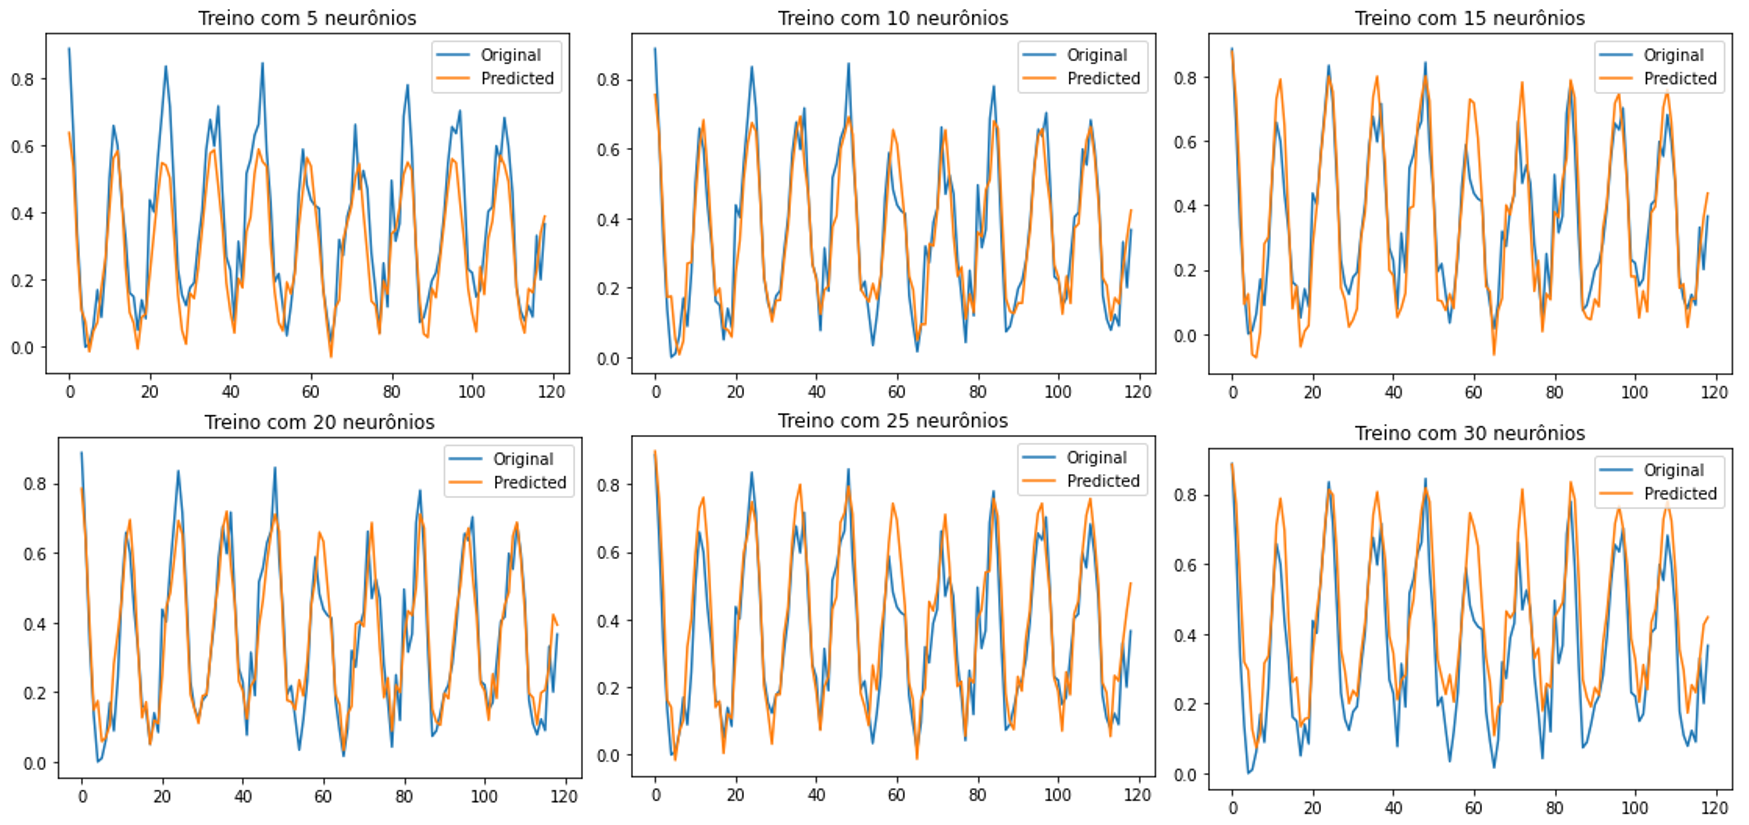
\includegraphics[width=0.9\linewidth]{Imagens/onestep/treinocomparadoneuronios}
		\caption{Comparação de Treinamento para diferentes quantidades de neurônios}
		\label{fig:treinocomparadoneuronios}
	\end{figure}
	\begin{figure}[H]
		\centering
		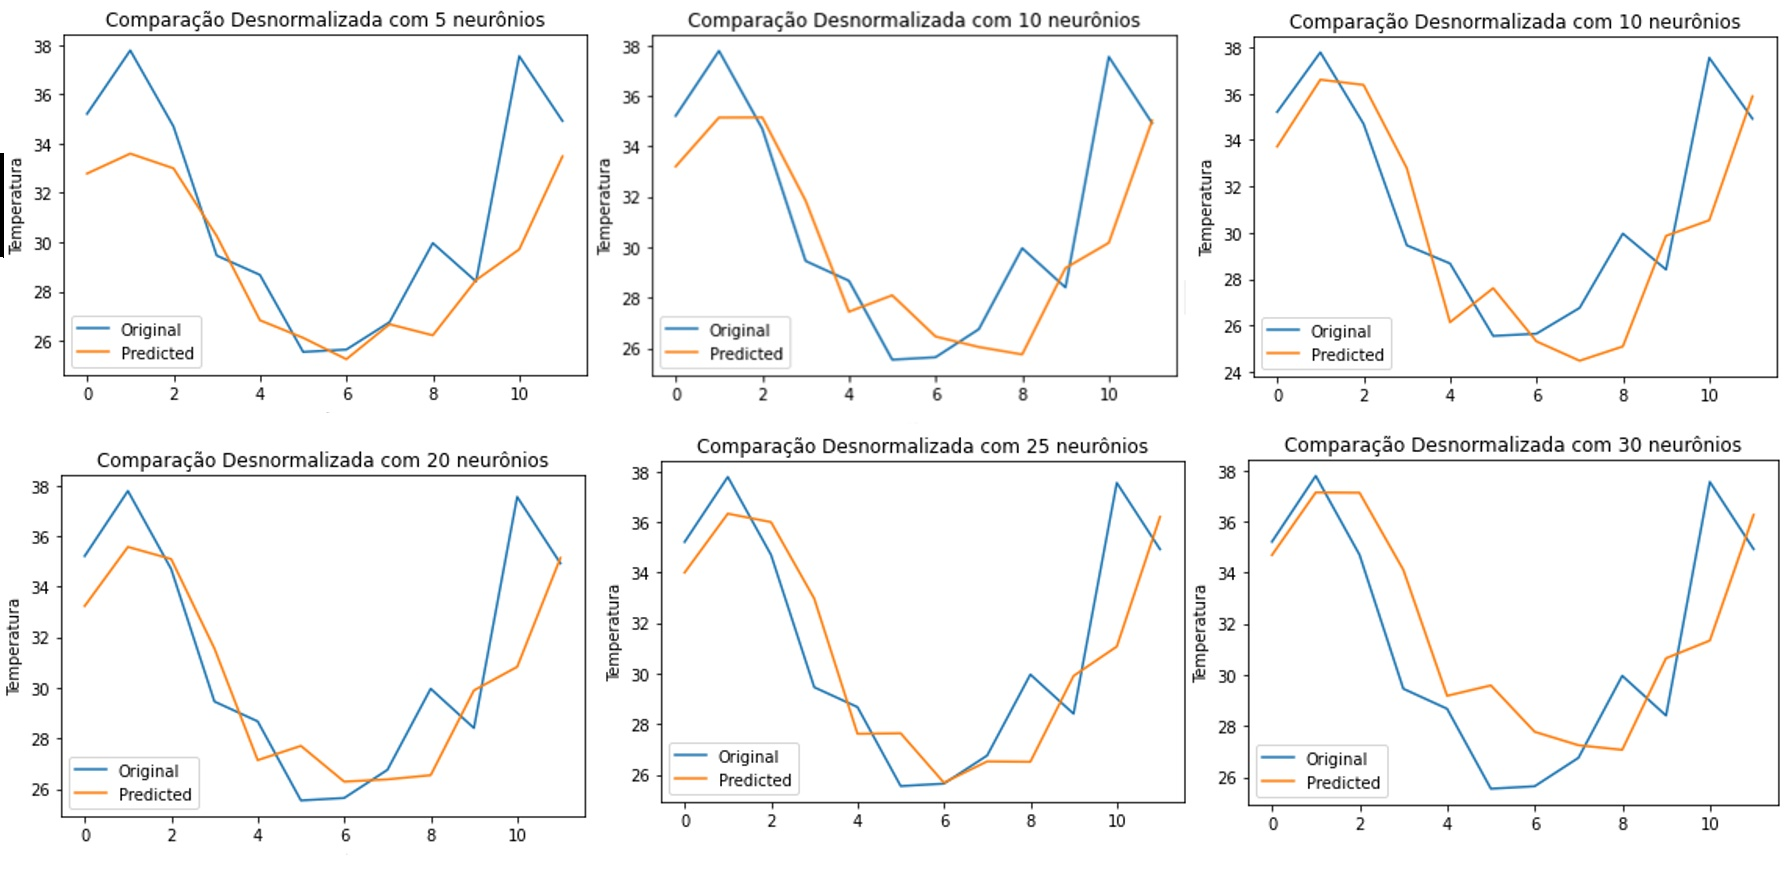
\includegraphics[width=0.9\linewidth]{Imagens/onestep/comparacaoneuronios}
		\caption{Comparação de testes para diferentes quantidades de neurônios}
		\label{fig:comparacaoneuronios}
	\end{figure}

	Com base na análise da tabela \ref{tab:comparacaoNeuronios} e das imagens \ref{fig:treinocomparadoneuronios} e \ref{fig:comparacaoneuronios}, percebe-se que para valores de 20 e 25 neurônios os erros são muito similares. Sendo assim, foi optado por eleger a rede com 20 neurônios na camada escondida por apresentar os melhores valores para as métricas analisadas e ser um modelo mais simples do que o de 25 neurônios.
	
	Podemos perceber perfeitamente, com as imagens acima, a importância da generalização e da especialização da rede. Note que para 5 neurônios a curva de treino e de teste é muito suave, o que indica que a rede não conseguiu aprender o suficiente por possuir poucos pesos treináveis. Ou seja, não adquiriu especialização. Por outro lado, com 30 neurônio a curva passa a ser desnecessariamente ruidosa devido à quantidade grande de parâmetros treináveis, causando perda de generalização.
	
	
	
	\subsection{Modifique a técnica de codificação mensal de ‘numérico’ para ‘binário’. Qual a mudança existente na arquitetura da Rede Neural? Analise o resultado (conjunto de treinamento e teste), usando as métricas RMSE e MAE.}
	
	As redes treinadas até então já estavam com a codificação mensal binária. Sendo assim, foi criado um modelo com exatamente os mesmos parâmetros da rede escolhida na seção \ref{subsec:2.1} mas com a codificação numérica para os meses. 
	

	
	\section{Previsão Multi-Step}
	
	\subsection{Implemente o processo de previsão multi-step}
	
	\subsection{Faça a previsão multi-step para o horizonte de previsão igual a 12 e compare com o resultado da previsão one-step.}
	
	\subsection{Modifique o tamanho da janela de entrada e avalie os resultados}
	
	\subsection{Modifique a topologia da rede para obter um melhor desempenho. Altere seus parâmetros (e.g. número de processadores na camada escondida, tipo de função na camada de saída) e avalie o desempenho em termos das métricas RMSE e MAE.}
	
	\subsection{Implemente a codificação ‘1 of N’ e use-a para modificar a representação da variável ‘mês’. Qual a mudança existente na arquitetura da Rede	Neural? Avalie o desempenho em termos das métricas RMSE e MAE.}
	

	\bibliography{bibliografia} 
	\bibliographystyle{plain}
\end{document}